\chapter{Programmets brugergrænseflade}
I dette kapittel vil programmet grafiske brugergrænseflade blive beskrevet.

\section{Login brugergrænseflade}
\begin{wrapfigure}{r}{0.5\textwidth}
    \label{img:login_interface}
    \vspace{-20pt}
    \begin{center}
        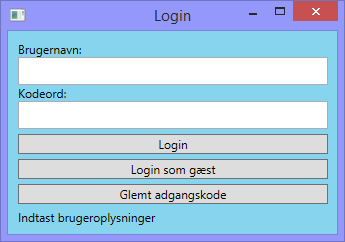
\includegraphics[width=0.48\textwidth]{UI/Login_Window_Empty_Fields.png}
    \end{center}
    \vspace{-15pt}
    \caption{Login interface}
\end{wrapfigure}
Login brugergrænsefladen (Figur \ref{img:login_interface}) er opstartsvinduet, og giver brugerne mulighed for at logge ind.
Formålet med dette er, at programmet skal kende identiteten af den person som anvender programmet.
Login knappen (samt at trykke på ``Enter''/``Return''-knappen mens tekstfelterne er i fokus), udfører et login. 
Forudsagt at brugeroplysninger angivet er korrekte, eller vises en passende fejlbesked.
Man kan også logge ind som en gæste bruge, som har reducerede tilladelser. 
Den kan bruges, hvis man vil tjekke noget infomation hurtigt, og ikke vil til at logge ind, da det tager tid.
Dette udføres ved at trykke på ``Login som gæst''-knappen. 

Efter fuldført login åbens et passene hovedvindue, med funktionaliteter i henhold til tabel \ref{tab:permissions}.

% LaTeX tabel som viser alle brugerniveauer og deres muligheder efter login.
% http://bit.ly/1kToHZ3 to edit raw table
\begin{table}
    \colorlet{shadecolor}{gray!40}
    \rowcolors{1}{white}{shadecolor}
    \begin{tabular}{l|llllll}
    ~                        & Gæst & Støttemedlem & Medlem & Elev & Underviser & Administrator \\ \hline
    Personlig forside        & ~    & ~             & \ding{51}     & \ding{51}    & \ding{51}          & \ding{51}             \\
    Se begivenheder          & \ding{51}    & \ding{51}             & \ding{51}      & \ding{51}    & \ding{51}          & \ding{51}             \\
    Tilmeld begivenheder     & ~    & ~	             & \ding{51}      & \ding{51}    & \ding{51}          & \ding{51}             \\
    Opret begivenheder       & ~    & ~             & ~      & ~    & \ding{51}          & \ding{51}             \\
    Se sejlture              & \ding{51}    & \ding{51}             & \ding{51}      & \ding{51}    & \ding{51}          & \ding{51}             \\
    Opret sejltur            & ~    & ~             & \ding{51}      & \ding{51}    & \ding{51}          & \ding{51}             \\
    Se logbøger              & \ding{51}    & \ding{51}             & \ding{51}      & \ding{51}    & \ding{51}          & \ding{51}             \\
    Opret logbog             & ~    & ~             & \ding{51}      & \ding{51}    & \ding{51}          & \ding{51}             \\
    Svar på logbog           & ~    & ~             & ~      & ~    & ~          & \ding{51}             \\
    Se undervisningstimer    & ~    & ~             & ~      & \ding{51}    & \ding{51}          & \ding{51}             \\
    Opret undervisningstimer & ~    & ~             & ~      & ~    & \ding{51}          & \ding{51}             \\
    \end{tabular}
    \caption{Tabel over alle brugerniveauer og deres tilladte funktioner.}\label{tab:permissions}\fixme{Måske skal denne tabel lige laves lidt om, enten indholdet, eller hvordan det virker i programmet.}
\end{table}

\section{Primære brugergrænseflade}
Det primære vindue tilgåes via login vinduet, som er det der starter ved programstart, eller logud. 
Der findes 4 vinduer, forskellen mellem dem er hvilke tabs der er aktive. 
I hver tab findes der en funktionalitet, samlet set findes følgende tabs:
\begin{itemize}% Denne skulle måske relatere til tabel tab:permission
    \item Forside
    \item Undervisning
    \item Begivenheder
    \item Medlemmer
    \item Både
\end{itemize}

Via hver af disse tabs, vil der være adgang til programmet forskellige funktionaliteter.
Der er også en log ud knap, som bruges til at vende tilbage til loginvinduet, således en anden bruger kan anvende systemet.
Programmet er lavet til at køre i opløsningen 1024x720 pixels.
Denne opløsning er valgt for at understøtte alt fra bærbare, med opløsninger som 1366x768 pixels i et vindue, og op til FullHD (1920x1080 pixels) osv.
Programmet har et lyst farveskema, men farverne hvid og en lys blå som hovedfarver (\#87D4EE).

\section{UserControls}
Der anvendes UserControls til at kode både brugergrænsefladen og den tilhørende code behind.

\subsection{Forside}
%\begin{wrapfigure}{r}{0.75\textwidth}
%    \label{img:frontpage}
%    \vspace{-20pt}
%    \begin{center}
%        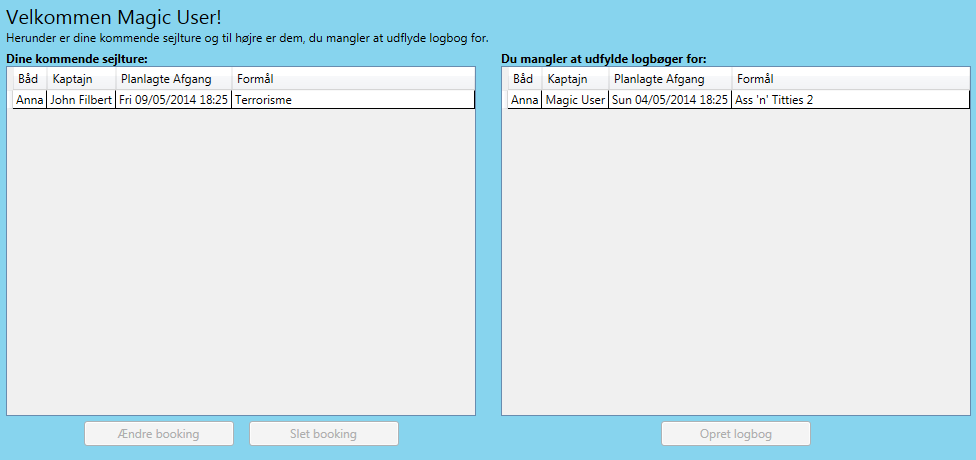
\includegraphics[scale=0.75]{UI/UserControl_FrontPage}
%    \end{center}
%    \vspace{-15pt}
%    \caption{Login interface}
%\end{wrapfigure}


\textbf{Datafremvisning:} 
En brugers kommende sejlture, og sejlture hvor brugeren mangler at udgylde logbøger for.

\textbf{Funktioner:} 
Kan åbne opret logbogsvinduet, enten ved dobbeltklik på sejltur, eller ved valgt af markering og tryk på opret logbog knappen. 

\textbf{Logik:} 
Hvis ingen sejltur er valgt i DataGridet med logbøger, så skal opret logbog knappen ikke være tilgængelig.

\fixme{Mangler billede, tænker at vi tager screenshots fra en platfor (win8/win7)}


\section{Vinduer}
\subsection{Opret sejltur}

\textbf{Datafremvisning:} 
Viser det data som bliver valgt, når brugeren vælger det. 
Der er også flere conscructorer, således der kan forudintastes data ved dets oprettelse.

\textbf{Funktioner:} 
Kan åbne vælg besætningsvinduet. 
Kan gemme data til databasen, hvis turen er gyldig.

\textbf{Logik:} 
Der verificeres om turen er gyldig, der er flere krav:
\begin{itemize}
    \item Er der valgt en båd?
    \item Er starttidspunktet efter det nuværende?
    \item Er sluttidspunktet efter starttidspunktet?
    \item Er båden ledig i dette tidsrum?
    \item Er der valgt mindst et besætningsmedlem?
    \item Er der valgt en kaptajn?
    \item Er der angivet et formål?
\end{itemize}

